\section{Simulation and Testing }

\begin{frame}
    \frametitle{Simulation Testing for Foundation DB}
    \begin{itemize}
        \item Testing and debugging distributed systems is challenging, particularly for Foundation DB.
        \item FDB employs an ambitious approach using a \textbf{deterministic discrete-event simulation}.
        \item The simulation environment quickly exposes bugs in the database, ensuring reproducibility for investigation.
    \end{itemize}
\end{frame}
%------------------------------------------------
% \begin{frame}
%     \frametitle{Deterministic Simulator}
%     \begin{itemize}
%         \item All database code is deterministic and multi-threaded concurrency is avoided (instead, one database node is deployed per core).
%         \item \textbf{All sources of non determinism and communication are abstracted}, including network, disk, time, and pseudorandom number generator
%         \item \textbf{Flow}, a syntactic extension to C++, facilitates deterministic execution of highly concurrent code.
%     \end{itemize}
% \end{frame}
%------------------------------------------------

\begin{frame}
    \frametitle{Flow, concurrency on C++}
    
\includegraphics[width=2cm]{img/3-Testing/cpp.png}

    \vspace{0.5cm}
   FDB needed to implement efficient asynchronous communicating processes with raw speed and I/O efficiency of C++.
\vspace{0.5cm}

Flow is an extention to the C++ 11 standard that is used to add async/await-like
concurrency primitives with automatic cancellation.

   
\end{frame}

%------------------------------------------------
% \begin{frame}
%     \frametitle{Execution of the Simulator}
%     \begin{itemize}
%         \item Workloads written in Flow interact with simulated FDB servers.
%         \item Multiple FDB servers communicate through a simulated network in a single discrete-event simulation.
%     \end{itemize}
% \end{frame}
%------------------------------------------------

\begin{frame}
    \frametitle{The FDB deterministic simulator}
    \begin{center}
        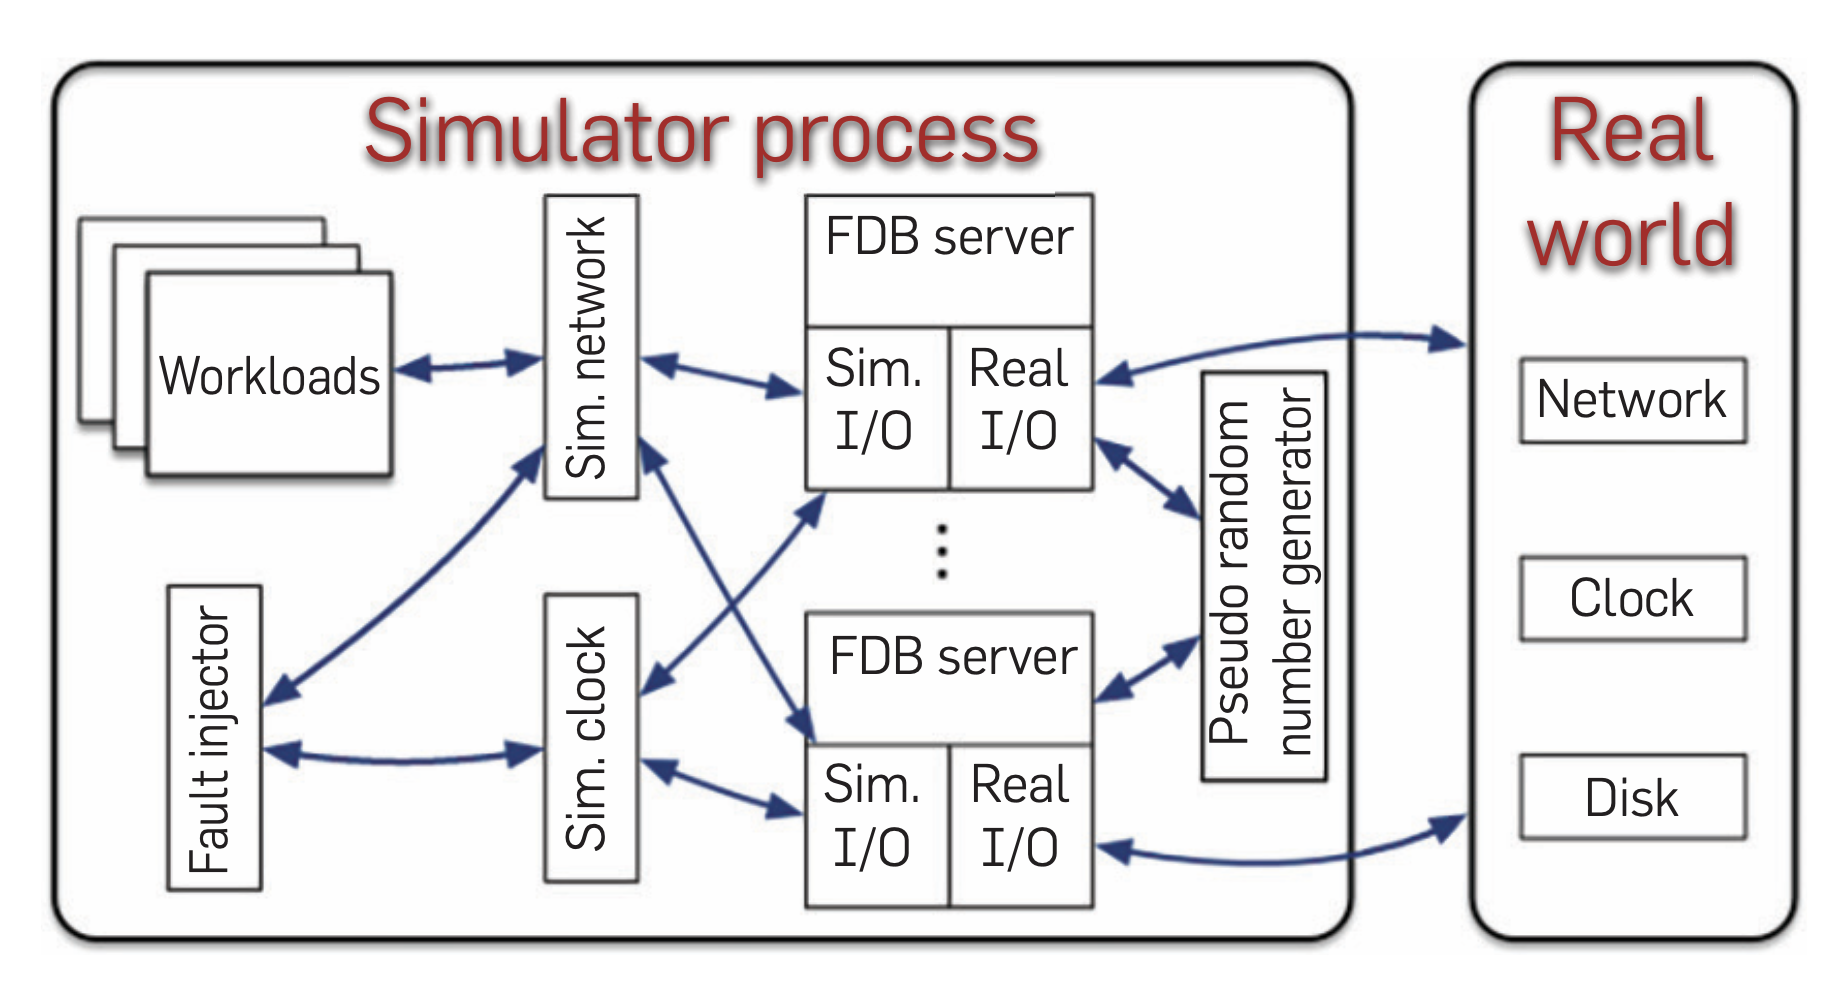
\includegraphics[width=0.8\textwidth]{img/3-Testing/The FDB deterministic simulator.png}
    \end{center}
    
\end{frame}
%------------------------------------------------


\begin{frame}
    \frametitle{Buggification: make rare states and events more common}
    Simulation is allowed to inject some unusual (\textbf{not contract breaking}) behavior such as 
    \begin{itemize}
        \item Unnecessarily returning an error from an operation that usually succeeds
        \item Injecting a delay in an operation that is usually fast
        \item Choosing an unusual value for a tuning parameter
    \end{itemize}
\end{frame}
%-------------------------------
\begin{frame}
    \frametitle{Limitations of Simulation}
    \begin{itemize}
        \item Simulation may not reliably detect performance issues or test \textbf{third-party dependencies}.
        \item Simulation cannot reliably detect performance issues, such as an imperfect load-balancing algorithm
    \end{itemize}
\end{frame}